\documentclass{article}
\title{Nechyba Ch.21 竞争性市场中的外部性}
\author{Dawei Wang}
\date{\today}
\usepackage{ctex}
\usepackage{amsmath}
\usepackage{amssymb}
\usepackage{graphicx} %插入图片的宏包
\usepackage{float} %设置图片浮动位置的宏包
\usepackage{subfigure} %插入多图时用子图显示的宏包
\begin{document}
	\maketitle
在证明非市场制度的合理性上,公平问题确实起到了重要作用,但基于某些条件,这些制度存在的原因更多的是源于效率而非公平。

即便市场是完全竞争的,仍然会有一些因素会导致市场在没有其他制度干预的情况下出现净损失,我们称这些因素为外部性(externalities)。当市场中的一方做出的决策对经济中另一个当事人产生了直接影响,而这些影响无法受市场价格所控制时,外部性就出现了。

例如污染这种行为实际上是具有社会成本的,但是这种社会成本并没有被市场定价。除非有其他制度去向厂商征收这笔成本,否则它将不在这些厂商的考虑范围之内。“外部的成本或收益”并没有被市场内在化的原因在于市场参与者不需要为它们进行支付。

\section{外部性问题}
外部性的基本特征是无论生产还是消费所带来的成本或收益都会直接地作用于非市场参与者。由于非市场参与者既不是商品的需求者也不是供给者,市场的需求曲线和供给曲线都不受这些外部性成本或收益的影响。这样作为价格承担者的消费者和生产者所组成的竞争性市场将继续在需求和供给相交均衡点进行生产。然而,尽管总边际支付意愿曲线仍然允许我们衡量消费者参与到市场上所获得的收益,供给曲线仍然允许我们衡量生产者产生的成本,但是现在增加了非市场参与者,他们也同样产生收益或成本。因而我们不能再简单地使用生产者和消费者剩余来衡量市场存在下的社会净收益。换言之,在计算总剩余时,我们需要把被完全竞争市场忽略掉的外部性成本和收益考虑在内。

由于在竞争性市场中每一个生产者的行为对于整个市场的影响是微乎其微的,所以个体生产者对整个污染的影响也是可以忽略不计的。因此我们可以将生产者看成是做供给决策时只考虑他们自己生产成本的个体,然后我们再将其中一部分受到总污染影响的生产者看作是一个独立的个体。

\hspace*{\fill}

生产外部性

\begin{figure}[H] %H为当前位置,!htb为忽略美学标准,htbp为浮动图形
	\centering %图片居中
	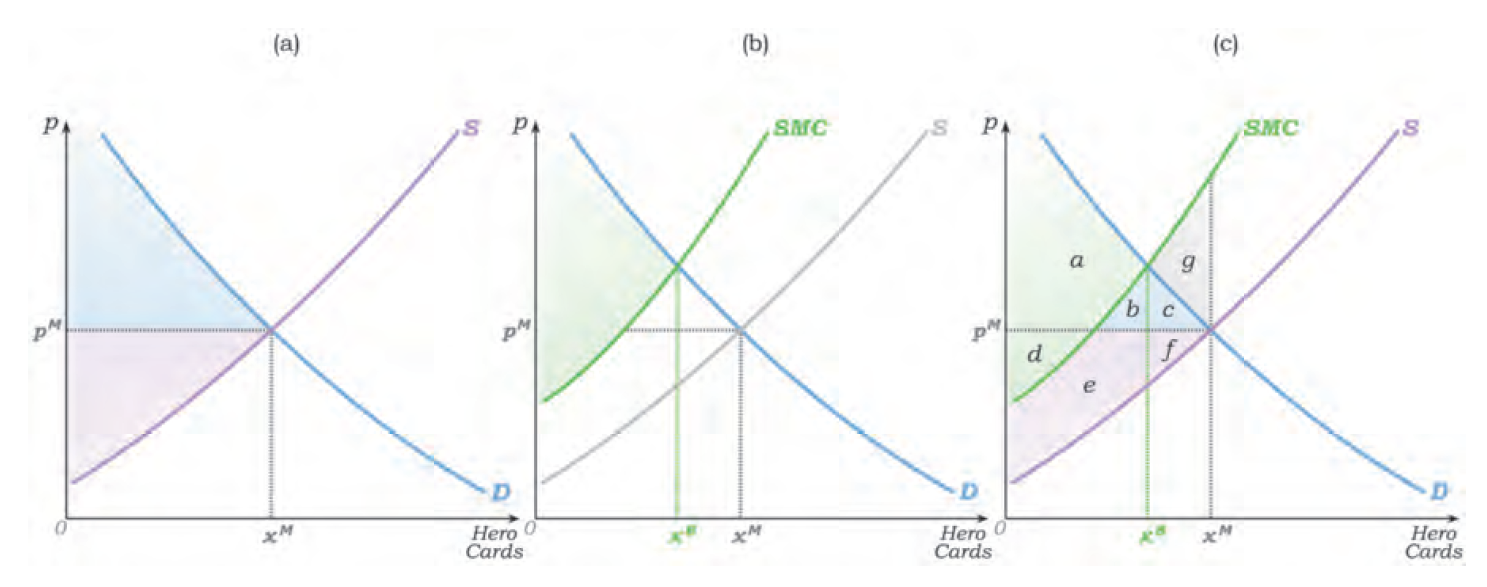
\includegraphics[width=1\textwidth]{21_1} %插入图片,[]中设置图片大小,{}中是图片文件名
	\caption{Maximizing Social Surplus in the Presence of a Negative Production Externality} %最终文档中希望显示的图片标题
	\label{Fig.main2} %用于文内引用的标签
\end{figure}

如果生产过程中出现了污染,那么每生产一单位商品都会向社会增加一单位污染成本,而这个成本既不由消费者承担也不由生产者承担。

组图(b)在组图(a)的基础上增加了一条“SMC”曲线。这条曲线代表生产的的社会边际成本(social marginal cost)。它不但包括由市场供给曲线所决定的生产者边际成本,而且还包括了强加于他人的额外成本。这样社会边际成本成本曲线一定位于供给曲线之上,因为它包括了生产者负担之外的成本。

若是一个全知全能的社会规划者来制定生产计划,则只要消费者边际支付意愿所表示的生产收益大于社会总的额外生产成本,则其会继续生产,一旦社会生产成本超过收益则其不会继续生产。

可以看到,寻求总剩余最大化的社会规划者将生产少于市场自发选择的产量。这表明在没有任何非市场制度缩减生产的情况下,市场将生产一个无效率的高产出水平。

在纯市场条件下,消费者剩余为a+b+c,生产者剩余为d+e+f,额外社会成本为b+c+e+f+g;在全知全能的社会规划者制定生产计划的条件下,消费者剩余和生产者剩余总剩余为a+d,额外社会成本为0。因此纯市场条件下的生产带来的净损失为g。

\hspace*{\fill}

另一种有效的税收

商品税是减少市场产出的一种政策工具。在不考虑外部性时它是无效率的,因为资源的市场分配在开始时是有效的,然而,在外部性存在的情况下无效率的产出的减少能够降低而不是增加净损失。

在生产负外部性存在的条件下,以减少市场产出来达到有效产量而征收的税,叫作庇古税(Pigouvian tax)。

\begin{figure}[H] %H为当前位置,!htb为忽略美学标准,htbp为浮动图形
	\centering %图片居中
	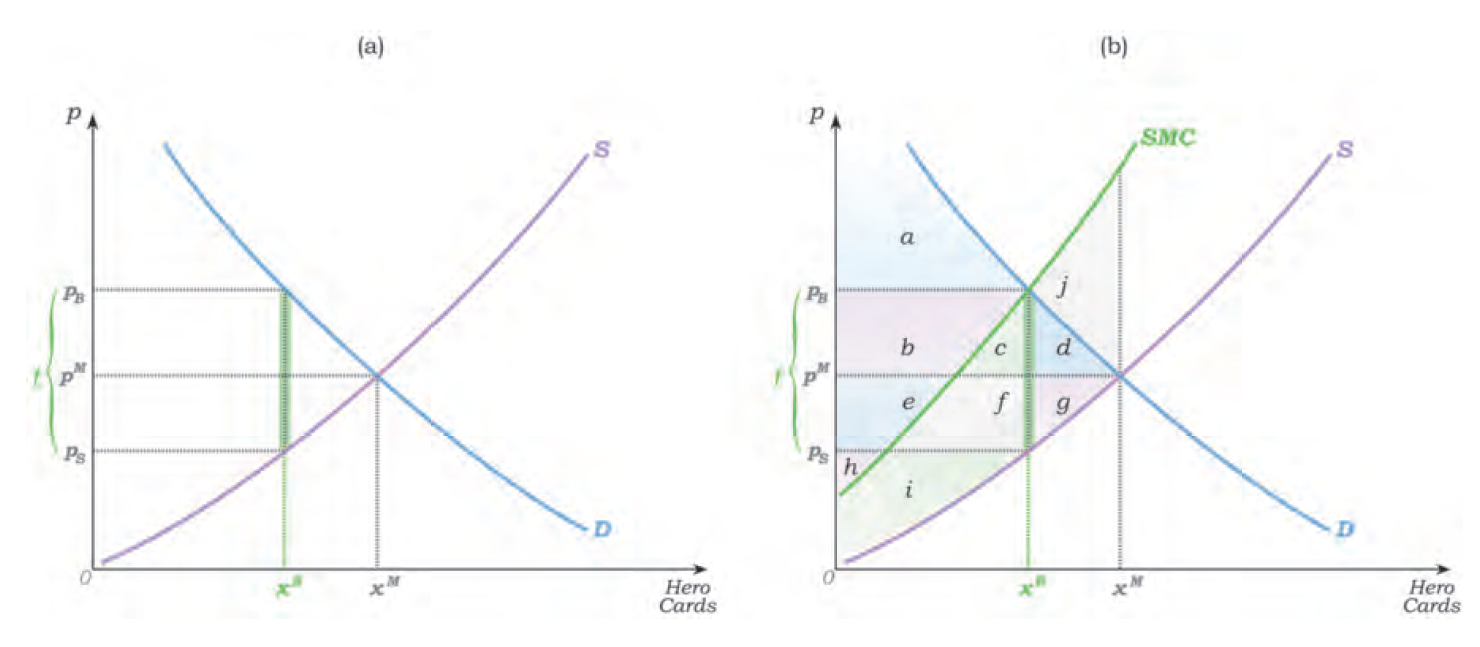
\includegraphics[width=1\textwidth]{21_2} %插入图片,[]中设置图片大小,{}中是图片文件名
	\caption{An Efficient Pigouvian Tax} %最终文档中希望显示的图片标题
	\label{Fig.main3} %用于文内引用的标签
\end{figure}

在税收t下,消费者剩余a和生产者剩余h+i与正的税收收入b+c+e+f及社会污染成本c+f+i结合在一起形成一个总剩余a+b+e+h。这与全知全能的社会规划者实现的最大化剩余完全相等,并消除了净损失i。

在不考虑外部性存在的情况下,税收的无效率是因为其扭曲了能协调生产者和消费者使其有效合作的价格信号,但是在外部性存在的情况下,价格信号已经扭曲到了它不能有效地协调生产与消费的程度。这时税收就消除了扭曲的问题,致使市场将“外部性内在化”。

为使政府能够征收有效的庇古税t,它必须清楚它想要市场达到的最有产量$ x^B $,以及在此产量上的市场的需求与供给曲线的差值。换言之,政府必须了解由最优产量上的污染所导致的社会边际损失。

原则上讲,让政府收集充分的信息去事实庇古税使市场恢复有效的生产并不是一件难事。然而假设现在有许多不同的产业都会产生污染。为设定庇古税,政府现在需要从每一个产业中了解这些相同的信息,然后为每个产业设定单位税。因为在最优条件下边际社会损失在每一点都是不同的,这就使得税率在这些污染产业之间变化不定。这将导致一个在各个产业中存在不同庇古税的复杂系统。而且随着技术的变化,这些税率也将不断调整。这样可能出现的最坏结果是:除非无论何时厂商自己找到减少污染的方法时政府都会相应地调整庇古税率,否则,每个产业中的个体厂商将不会从自发应用减污技术中获得任何收益,因为它们仍要面对与之前相同的税率。因此庇古税征收起来理论上简单,实际上复杂。

出于这个原因,大多数经济学家都不会推荐对产出征收庇古税,作为代替,他们会转向更直接地驱使生产者对减少污染还是支付污染的社会成本作出权衡地方法。这种关注焦点地改变在新技术的作用下是可能实现的,该技术要允许政府准确定位是谁在排放污染,进而要求污染者直接为污染进行支付。这既可以通过一种污染税(pollution tax)(与向产出征收的庇古税相反),又可以通过设计市场为基础的政策来实现。

\hspace*{\fill}

以市场为基础的环境政策

政府确定一个可接受的总污染水平(包括每一种污染),然后发放允许所有者每周排放一定量不同种类的污染物的文件。这些文件被称为污染许可证(pollution vouchers)或可交易污染许可证(tradable pollution permits),代表在一定程度上“可以污染的权利”。然后政府就通过拍卖或简单地下放给不同产业地不同厂商来释放这些权利。政府采取何种方式分配这些许可证被证明是无关大局的,重点在于拥有这些许可证地个体可以向其他个体卖掉它们,如果他们愿意这样做的话。本质上,这个政策通过调整并限定污染许可证地数量对污染进行“总量管制”,又允许许可证的“交易”以决定谁可以排放它们,因此就出现了被称为限额交易(cap-and-trade)的政策。

污染许可证对生产者来说是有价值的,因为它允许生产者在他们的生产过程中排放污染。同时,无论何时生产者选择去使用许可证,都会产生一个经济成本,因为他本可以选择将这个许可证出卖给其他人。同时若一个个体减污技术使用越多其对污染许可证的需求越小,从而可以达到使用减污技术节省成本的目的。通过向经济中引入污染许可证,政府就制造了一个新的市场,污染许可证市场。

\begin{figure}[H] %H为当前位置,!htb为忽略美学标准,htbp为浮动图形
	\centering %图片居中
	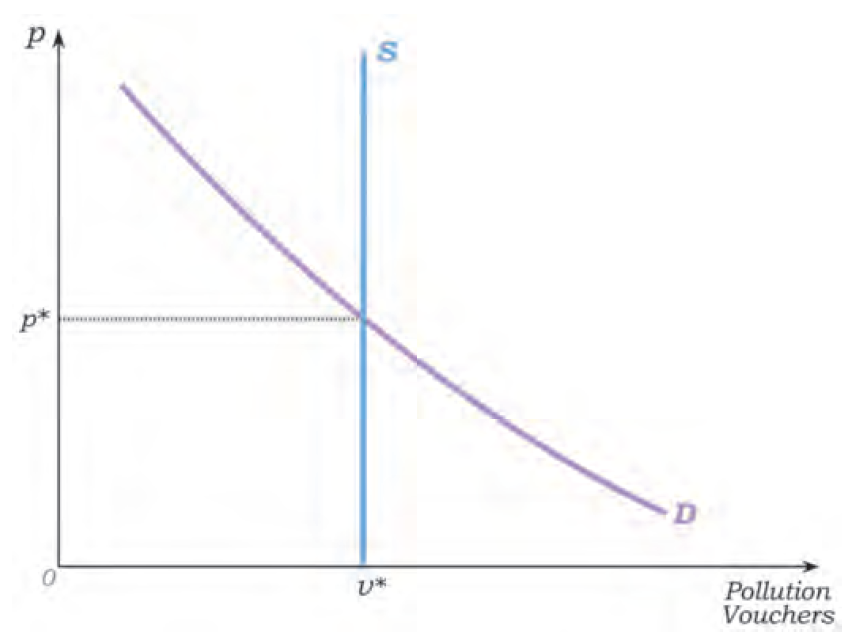
\includegraphics[width=1\textwidth]{21_3} %插入图片,[]中设置图片大小,{}中是图片文件名
	\caption{A Market for Pollution Vouchers} %最终文档中希望显示的图片标题
	\label{Fig.main4} %用于文内引用的标签
\end{figure}

污染许可证市场的供给是完全无弹性的(由政府控制污染许可证数量),在生产过程中排放污染的厂商是这些许可证的需求者,需求的大小取决于生产不同类型产品时需要排放多少污染,以及这些厂商通过各种手段减去生产污染排放的难易程度。

假设政府能够有效地监督污染的产业,污染许可证系统会达到以下效果:首先,污染者需要为他们排放的污染购买足够的权利,这就为他们增加了一个成本,由于污染许可证成为了生产过程中的一项投入,使厂商的MC曲线向上移动,这又改变了污染产业的市场供给曲线,进而导致了在这些污染产业中更少的产出。其次,该系统为厂商寻找(或投资)减污技术提供了一种激励。最后,这个系统为独立研发减污技术的新厂商的出现创造了激励。这个系统增加了对这种科技的需求,否则污染者为了生产就不得不为购买污染许可证而进行支付。

作为结果,该系统在社会成本最小化点达到了污染的全面降低,且政府不需要对条件的变化作政策的调整。新生成的许可证市场就会使那些已得到许可证的,没得到许可证的,因降低污染成本过大而选择使用许可证的和其他选择以更低廉价格减污技术的厂商相互配给供应。换句话说,污染许可证是这样一种政府干预行为,政府在可能成本最小化及排除进一步干预的前提下,利用新建立市场的力量来获取降低污染所需要的信息。

最后:尽管污染许可证为用最低的成本使污染减少到目标水平提供了一个机制,但污染许可证系统不能保证一开始就设定出社会最优的污染目标。如果确定这个目标的政治程序是有效的,那么目标就是被最优设定的。否则,目标可能太高或太低。限额交易系统为我们所做的全部就是帮助我们以最少的成本达到目标。

\hspace*{\fill}

污染税、庇古税和限额交易

直接向污染征税与庇古税有相同的优势,在限额交易系统中我们就指出过这一点,如果每单位污染税税率是与在限额交易系统中出现的每单位污染物价格一致的话,那么污染税实际上就等同于建立可交易污染许可证。两个系统都为厂商投资减污技术提供了激励,而且都不需要政府随环境变化而调整税率(在对产出征收庇古税中出现的处境)。另外,除非政府对有效税率或有效污染许可证的数量充分掌握信息,否则两种系统都不会自动形成完全有效的结果。

\subsection{消费外部性}

外部性可以在生产中出现,也可以在消费中出现,并且它既可以是积极的,也可以是消极的。这些论断的本质是相同的,除了消费者从消费中直接获得私人收益外,社会中其他个体也会通过非市场定价的方式间接地获得收益。

\hspace*{\fill}

消费正外部性

\begin{figure}[H] %H为当前位置,!htb为忽略美学标准,htbp为浮动图形
	\centering %图片居中
	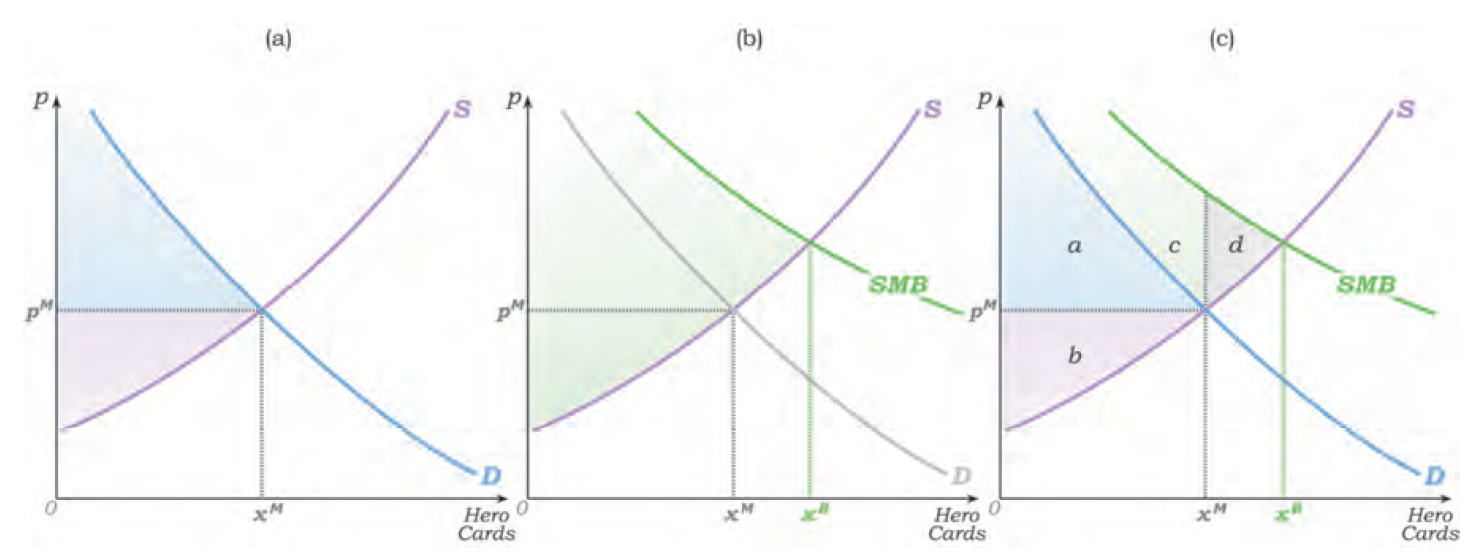
\includegraphics[width=1\textwidth]{21_4} %插入图片,[]中设置图片大小,{}中是图片文件名
	\caption{Underproduction in the Presence of a Positive Externality} %最终文档中希望显示的图片标题
	\label{Fig.main5} %用于文内引用的标签
\end{figure}

在组图(b)中引入了一条新的SMB曲线,或者称为社会边际收益(social marginal benefit)。这条曲线包含了社会中每单位消费中获得的全部收益。

纯市场机制下的社会总剩余为a+b+c;在全知全能的社会规划者制定的产出水平下社会总剩余为a+b+c+d。因此在没有非市场制度引导额外生产的情况下社会会产生一个净损失d。

\hspace*{\fill}

庇古补贴

当补贴用于“内在化”正外部性时,就被称为庇古补贴。就像在征税时的情形一样,它能够使被外部性扭曲的市场价格恢复效率。

\begin{figure}[H] %H为当前位置,!htb为忽略美学标准,htbp为浮动图形
	\centering %图片居中
	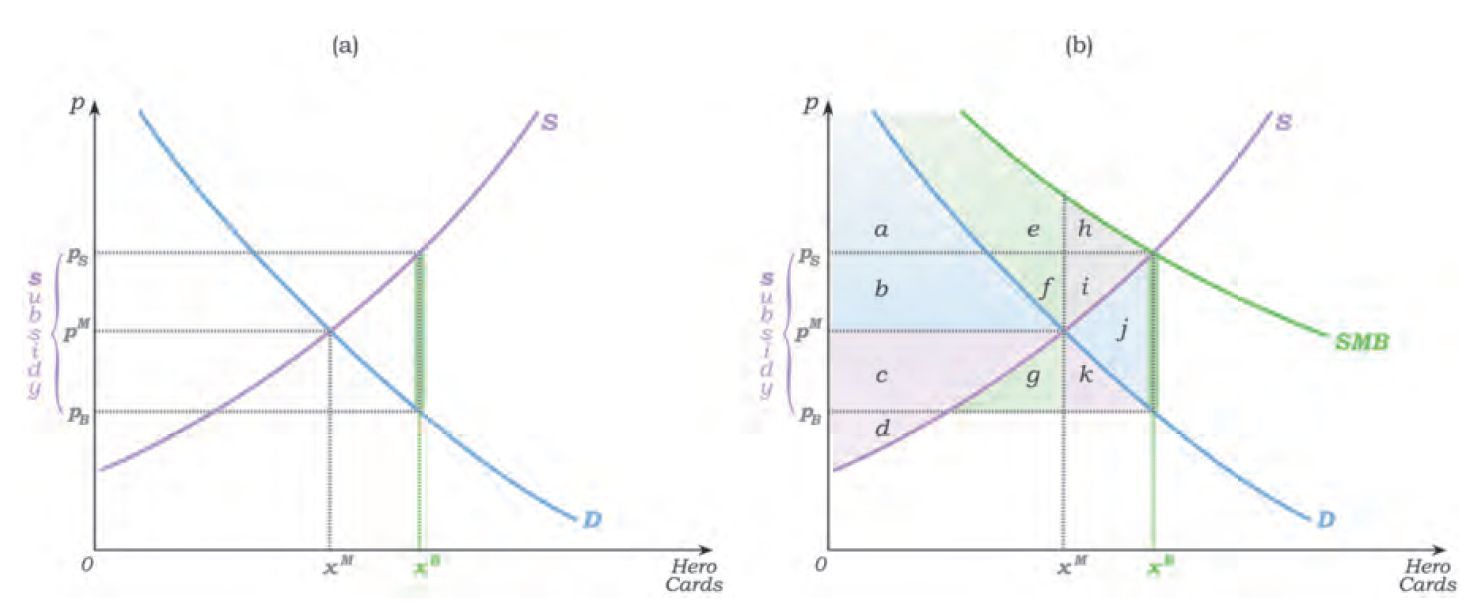
\includegraphics[width=1\textwidth]{21_5} %插入图片,[]中设置图片大小,{}中是图片文件名
	\caption{An Efficient Pigouvian Subsidy} %最终文档中希望显示的图片标题
	\label{Fig.main6} %用于文内引用的标签
\end{figure}

在补贴之前,消费者和生产者剩余即a+b+c+d,非市场参与者得到额外剩余e+f。这样纯粹市场分配的总剩余就为a+b+c+d+e+f。在有补贴时,消费者剩余为a+b+c+g+k,生产者剩余为b+c+d+f+i,非市场参与者剩余为e+f+h+i+j,补贴成本为b+c+f+g+i+j+k,得到的总剩余为a+b+c+d+e+f+h+i。这样就实现了社会最大可能性收入,补贴消除了在纯粹市场分配中出现的净损失h+i。

\hspace*{\fill}

慈善捐赠、政府政策与公民社会

政府可以通过创造新的污染许可证市场来有效地将污染减少到政府设定的某一水平上,而不是每年都要计算正确的庇古税,然而对于消费正外部性而言,现实中缺乏类似的市场政策。

公民社会制度时发生于政府环境和显性市场价格之外的个体之间的相互作用的集合。这种制度更多地出现于个体劝说而不是政治程序,用来解决大家关注的市场无法解决的问题。

正如污染许可证代表政府对应用市场实力寻找解决过度污染问题的有效方法做出的努力,政府也经常会让公民社会制度参与进来。例如针对对从事慈善事业的资金进行税收减免。这样当政府在为每个可以产生正外部性的产业设计明确的补贴面临太多困难时,它可以提供这种一般性补贴,旨在为公民社会机构寻找非市场、非政府解决方案时减少困难。

\hspace*{\fill}

\subsection{外部性:市场失灵或市场存在的失败?}

污染和市场缺失

考虑市场里污染是生产副产品的情形。在这种情况下市场会过量生产的原因是生产者没有被迫去承担他们做生产决定时施加于社会的全部成本。如果生产过程中每一种被用到的投入都有各自的市场,包括“干净空气”市场,那么生产者必须支付他们造成的全部成本。因此空气污染作为一个一直市场效率的问题的出现是因为生产中这种投入不是被买来的。

外部性之所以是一个问题就是因为我们无法找到一种创造干净空气市场的方法。如果有这样一个市场,且如果所有的空气都被不同人群拥有,那么所有干净空气的使用者都将为其使用进行支付。这样干净空气的市场将进而导致一个市场价格,并且在任何其他的外部性不存在的情况下,达到在干净空气的市场的社会剩余最大化。生产者的边际成本曲线将上移,市场供给曲线上移并等于生产的社会边际成本(SMC),而不是排除了污染社会成本的私人边际成本。

在一个抽象的概念意义上说,外部性的存在产生的市场失灵可能要追溯到市场存在的失败。

\hspace*{\fill}

公地悲剧

政府的一个大的作用就是更普遍地去行使权力使市场更有效。我们一直以来对待市场效率都做了一个隐含的假设,那就是市场对各种诸如劳动和资本的投入都是实际存在的。假设这样的市场存在并假定个体有可以交易的资源,这就假定了有一个特定的机制可以保护拥有资源的个体的产权。需要一个建设完备的法律上生效的产权系统,而且这一系统实际上需要政府的保护以及一个完备的法律系统去捍卫产权。

外部性,产生于这些产权还未被建立。污染的问题源于对于干净空气不存在一个产权系统去强迫厂商为它们在生产中作为投入使用的干净空气进行支付。无论何时,只要一种资源没有明确地归属于某人,这就可能使一些经济主体占用这些资源并且不支付成本,即便这向社会施加了成本。它进而产生了一个逻辑结果:如果政府建立一个当前无明确归属资源的产权系统是可行的,那么政府干预就能够创造出一个新的市场,该市场能够通过强迫市场参与者去面对他们的真实社会成本而减少外部性所带来的问题。

因此,经济学家把由市场缺失所导致的外部性问题称为“公地悲剧”(Tragedy of the Commons),当资源是“公共”的而不是私人拥有时,社会损失的“悲剧”就出现了。

\hspace*{\fill}

道路拥挤

道路拥挤问题是公地悲剧的一个例子。道路,大体上说是公共所有的,也就是并不属于任何人。当我们来到道路上时,我们可能会考虑到道路的关卡成本、我们时间的成本、我们使用的汽油以及我们车辆的折损成本。然而,我们没有考虑我们施加到其他每一个在路上的人的成本。换言之,我们每一个人都对其他每一个在道路上的人施加了一个负外部性,因为我们都增加了道路的拥挤程度。在没有一个我们面对由我们自己的私人行为所产生的社会成本的机制时,我们将倾向于多次的行驶,而我们将在“错误”的时间出现在道路上。

对拥挤道路的驾驶进行定价更直接地通过过路费的方式施行。

\hspace*{\fill}

较小的外部性、法庭与科斯定理

讨价还价、交易成本和科斯定理

科斯定理表明:在存在负外部性的情况下,产权的清晰界定是基本条件;但这些产权具体如何界定并不是基本条件。我们需要做的全部就是去决定谁拥有权利,然后让人们通过谈判自行解决问题。

当产权界定后解决外部性问题的障碍被称为交易成本(transactions costs),并且如果它们足够高的话,谈判就失去了机会。在足够高的交易成本存在的情况下,法官需要弄清有效的结果是什么并相应地进行裁决,这样就没有必要进行谈判。

完整的科斯定理的表述:如果交易成本足够低的话,只要产权足够清晰,那么外部性存在时的有效结果就会出现。

我们进而看到只要交易成本足够低,科斯定理对于我们解决外部性问题来说是一个转移矛盾的方法,而当更少的人受外部性影响后交易成本会变得更低。因此我们可能不需要为每天都要发生的只会影响少量人的外部性而担忧。相比于只要掌握少量信息的政府去做行政命令而获得有效结果,人们自行解决而获得有效结果的可能性要大得多。换言之,如果外部性问题需要在法庭上作出裁决,只要在“小的外部性环境”下的人们对法律如何对待外部性问题有合理的预期,那么这些问题的最好的解决方式就是在通常的定价-管制市场背景之外的公民社会中由人们自发地相互完成的。













































	
\end{document}